\chapter{基于RNN的深度强化学习混合模型在直接营销场景中的研究}
% 首先介绍直复营销问题使用强化学习研究的现状(函数逼近存在的问题,以及现行的解决方案和思路,从而引出本文的方法思路)
% 介绍深度强化学习
% 介绍本文提出的混合网络模型算法

%  在中文中,直复营销和直效营销指代的是同一概念, 但是从英文来看是不一样的, 实际上我们有两个单词:Direct Response Marketing 和 Direct Marketing, 相较于Direct Response Marketing, Direct Marketing的概念更基础和广阔,指代不通过第三方,中间人,从而直接对客户进行推广和营销,也就是寄送购物目录等一系列下文出现的手段,在这些不同的手段中,我们有一些叫做直接反应xx的手段,其实他们就属于 Direct Response Advertising 的范畴,讲究的是快速直接的获得客户的回应, 而 Direct Response Marketing 就是在此基础上衍生的,但是因为没有专人进行系统的分类和定义(也有可能已经有分类,还没有普及),现在他们两个由于本身概念的一定重合,使得很多人出现混淆,在维基百科中文版或者百度百科上都没有系统的分出两者,更不曾提到有两个概念,很容易误导别人。随着时代和市场的发展迟早会出现更系统更科学的分类,让我们拭目以待。

在直接营销的场景中,企业以追求客户的生命周期价值最大化为目标,这与强化学习以追求累计奖赏最大化的目标不谋而合。另外,在该场景中,企业需要在较长的时间内不断的与顾客直接进行营销交互,属于序列决策问题,并且因为该场景的复杂性,还存在用户状态部分可观测的问题。而以RNN为代表的循环神经网络除了可以利用自身特有的循环结构巧妙的处理序列问题外,还可以利用神经网络自动的学习隐藏状态的表达方式。所以,结合以上两方面,本章提出了基于RNN的深度强化学习的混合模型。在该模型中,使用RNN网络来学习和提高针对隐藏状态的表征能力,然后利用DQN网络逼近Q值函数,充分利用了两个网络模型的各自优点。另外,为了提高训练时收敛的速度和精度,又提出了两种改进的混合网络模型:一步混合模型1-RNN+DQN和两步混合模型2-RNN+DQN。

\section{直接营销问题阐述}
在本部分中,我们首先对直接营销问题做了进一步介绍,明确所研究问题的场景以及特点,然后说明了直接营销场景的目标是追求客户终身价值,并且存在状态部分可观测的问题,由此引出了本章使用深度强化学习作为该问题的解决方法的原因。

\subsection{直接营销场景}
直接营销即企业可直接得到客户回应状况的营销方式,是客户关系管理中的一项重要议题。具体来说就是指企业企图直接通过可确定地址的媒体向客户传递沟通信息,以寻求对方直接回应(问询或订购)。它强调与客户直接对话,并注重掌握受众信息,以此为据建立长期关系,提高受众的忠诚度,达到重复购买的效果。直接营销不同于通常的广告传播,它并不借助第三方媒体,也不在公开市场上、大众广告栏或者广播电视媒体上传递信息。商品或者服务的信息直接定位于目标客户。主要的应用场景包括通过邮寄、电子邮件或者面对面沟通。另外,在当今互联网时代的广告业务中,针对用户进行的个性化广告推荐推送服务的精准营销,正是属于直接营销问题的范畴,因此解决好该问题具有很高的社会商业价值。

在该场景中,企业需要通过与客户进行长时间的营销交互,然后结合所采取的营销行为和客户的响应情况进行分析,以此来判断客户对营销产品的喜好,进而可以辅助企业进行之后的营销决策,维护企业与客户之间的良好关系。具体来说,在每个需要进行营销的时刻点,企业会对客户采取营销行为,比如发送宣传单、促销广告或者优惠券等营销信息,作为反馈,客户可能会访问该企业的相关资讯或者会完成一定金额的订单又或者会简单的忽略掉此次的营销行为。所以,企业需要在进行营销活动之前做出要对哪些目标客户进行营销的决策,以使的企业可能产生的收益最大化。

\subsection{用户生命周期价值}
客户终生价值(Life-Time Value, LTV)指的是每个客户在未来可能为企业带来的收益总和,通常被应用于市场营销领域。研究表明,如同某种产品一样,客户对于企业利润的贡献也可以分为导入期、快速增长期、成熟期和衰退期。

在直接营销场景中,假如企业在某一时刻对某一客户采取了营销行为,客户可能会即刻给出反馈信息,也能会过了很长时间才会产生反馈信息,也可能会在之后给出多次的反馈信息。也就是说,营销行为对用户的影响是长期的而且用户对营销行为的反应是存在延迟的。所以,在直接营销场景中,企业通常把最大化用户生命周期价值作为评价营销效果的重要指标。通过第二章的介绍,我们知道强化学习在学习过程中考虑了延迟奖赏,并且以追求累计回报最大化为目标,所以直接营销问题就可以自然的表述为一个基本的强化学习问题。其中,即时利润看作是奖赏,LTV看做长期的价值函数(回报)。文献\citep{tkachenko2015autonomous,pednault2002sequential,silver2013concurrent}都正是以此想法为出发点,将强化学习技术应用在广告营销中,并且取得了较好的表现。

\subsection{部分可观测问题}
然而,与机器人和人机交互等现实应用场景中所面临的问题类似,在直接营销的场景中,客户的状态(马尔科夫状态)是部分可观测的,这会影响强化学习技术在这些场景中的应用表现。根据马尔科夫的无后向性,我们知道,客户的当前状态完全概括了他与企业在此之前的整个交互历史,也就是说客户的未来响应情况与之前的交互历史无关,只和当前状态和未来的所采取的营销行为有关。然而,在直接营销这种复杂的现实场景中,构建这种具有马尔科夫性的状态是很难的。即使像在直接营销中比较常用的Recency-Frequency-Monetary用户价值模型\citep{tkachenko2015autonomous},也仅仅捕获到了客户真实状态中的部分信息。因此,对这些场景使用强化学习之前,进行隐藏状态的推断表示是很重要的。

在强化学习的研究和应用中,处理部分可观测状态最常用的方法是使用部分可观测的马尔科夫决策过程(Partially Observable Markov  Decision Process,POMDP)\citep{kaelbling1998planning},并且已经在一些诸如机器人、人机对话等领域取得了不错的表现\citep{pineau2003point,williams2007partially}。在POMDP中,因为agent对环境观测的局限性,所以在应用过程中多了一步agent对当前所处状态可信度的判断,
但是,对可信度的判断需要借助领域专家自定义的隐状态表示方法,而这些领域知识在一些复杂的现实应用中是很难获得的。

近年来,深度强化学习成功应用在了游戏、围棋等领域。它们主要是将强化学习技术和深度神经网络相结合,其中,利用神经网络在推断学习系统环境的复杂特征的同时更好的逼近价值函数。与POMDP不同的是,深度神经网络可以在不依靠专家领域知识的前提下,对任何给定的问题都可以自动的给出隐藏状态的合理表示方法\citep{deng2014deep},从而解决了在设计隐状态时所面临的困扰。以上就是本文选择使用深度强化学习解决直接营销问题的出发点,特别的,我们对现有的网络结构做了近一步的改进优化。

\section{深度强化学习}
近年来,深度强化学习之所以引起了学术界和工业界的广泛关注,是因为DeepMind团队利用所提出的Deep Q-learning Network(DQN)算法成功的应用在了雅达利(Atari)游戏和围棋等领域。同样,本章所提出的基于RNN的深度强化学习混合模型也是基于DeepMind团队的DQN模型。所以。本部分在总结了DeepMind团队于2013年在NIPS\footnote{Conference and Workshop on Neural Information Processing Systems,神经信息处理系统大会}发表的论文\citep{mnih2013playing}和2015年在Nature发表的论文\citep{mnih2015human}的基础上,对DQN模型的创新点进行详细介绍。

\subsection{Q-learning}
在算法$\ref{algo:algorithm_2}$中,我们对Q-learning算法做了详细介绍,Q-learning用到的思想是主要是异策略和时间差分方法。

异策略,就是指的行为策略(产生数据的策略)和要评估的策略不是同一个策略。在算法$\ref{algo:algorithm_2}$中,行为策略是第6行的$\epsilon-greedy$的策略,而用于评估和改善的策略是第7行的贪婪策略(每个状态取值函数最大的那个行为)。时间差分方法,是指利用时间差分目标来更新当前行为的值函数。在Q-learning中,时间差分的目标就是$r+\gamma \max_{a} Q(s_{t+1},a)$。

在传统的Q-learning方法中,当状态和行为空间是离散的且维数不高时,我们一般使用Q-表(矩阵)的形式储存每个状态行为对的Q值。但是,当状态和行为空间是高维连续时,就会对存储空间提出很大的要求,使用Q-表不现实。比如在在围棋中有$10^{170}$种状态,在Atari游戏中有$256^{210\times160}$种状态。通常解决方法是把Q-表的更新问题变成一个函数拟合问题(参见第二章),可以从相近的状态得到相近的输出动作。如公式$\eqref{seq_2_3_2}$所示那样,通过更新参数向量$\mathbf{\theta}$使Q值函数逼近最优Q值。但是,普通的线性函数在函数逼近值,往往会会因为表征能力不够而影响逼近效果。

幸运的是,深度神经网络主要的优势之一就是可以自动提取复杂的特征,从而可以高效的解决高维且连续的问题。因此,出现了基于深度学习的深度强化学习(Deep Reinforcement Learning, DRL)技术。在众多DRL模型中,以DQN模型最具代表性,因为它解决了DRL中一些一直以来悬而未解的关键问题,才使得深度强化学习以惊艳的表现重新回到大众的视野中。

\subsection{DQN}
 深度神经网络和强化学习技术的结合,虽然可以在一定程度上达到优势互补的作用,但是也面临着许多问题。1)深度学习需要大量带标签的样本进行训练,而强化学习只有奖赏的返回值,而且存在延迟等问题。2)深度学习的样本之间是独立的,且目标分布是固定的,而强化学习前后的状态是相关的,并且目标分布在一直变化。3)就像第二章提到的那样,使用非线性网络进行值函数逼近时,往往会出现收敛不稳定等问题。

 面对以上问题,DQN提出了对应的解决方法。1)通过Q-learning使用奖赏来构造标签,并且使用卷积神经网络进行值函数的逼近。2)通过经验回放(Experience Replay)机制来解决强化学习中相关性以及非静态分布的问题。3)通过设置独立目标(Target)网络来单独处理时间差分算法中的TD偏差,进一步降低数据之间的关联性,从而削弱收敛不稳定的问题。本部分,针对以上改进方法进行详细介绍。

 \paragraph{卷积神经网络逼近值函数与构造标签}
图\ref{fig:CNN_DQN}为DQN模型逼近Q值函数时所使用的深度卷积神经网络的结构,它包含两个卷积层加两个全连接层。利用神经网络逼近值函数属于参数化的非线性逼近方法,不仅具有很强的表征能力,而且还可以自动自动提取复杂的特征。此处的值函数对应着一组参数,也就是神经网络中每层网络的参数,我们可以用向量$\mathbf{\theta}$表示,对应的值函数可以表示为$q(s,a;\mathbf{\theta})$,所以对值函数的更新也就是对参数向量$\mathbf{\theta}$的更新。
\begin{figure}[htbp]
\centering
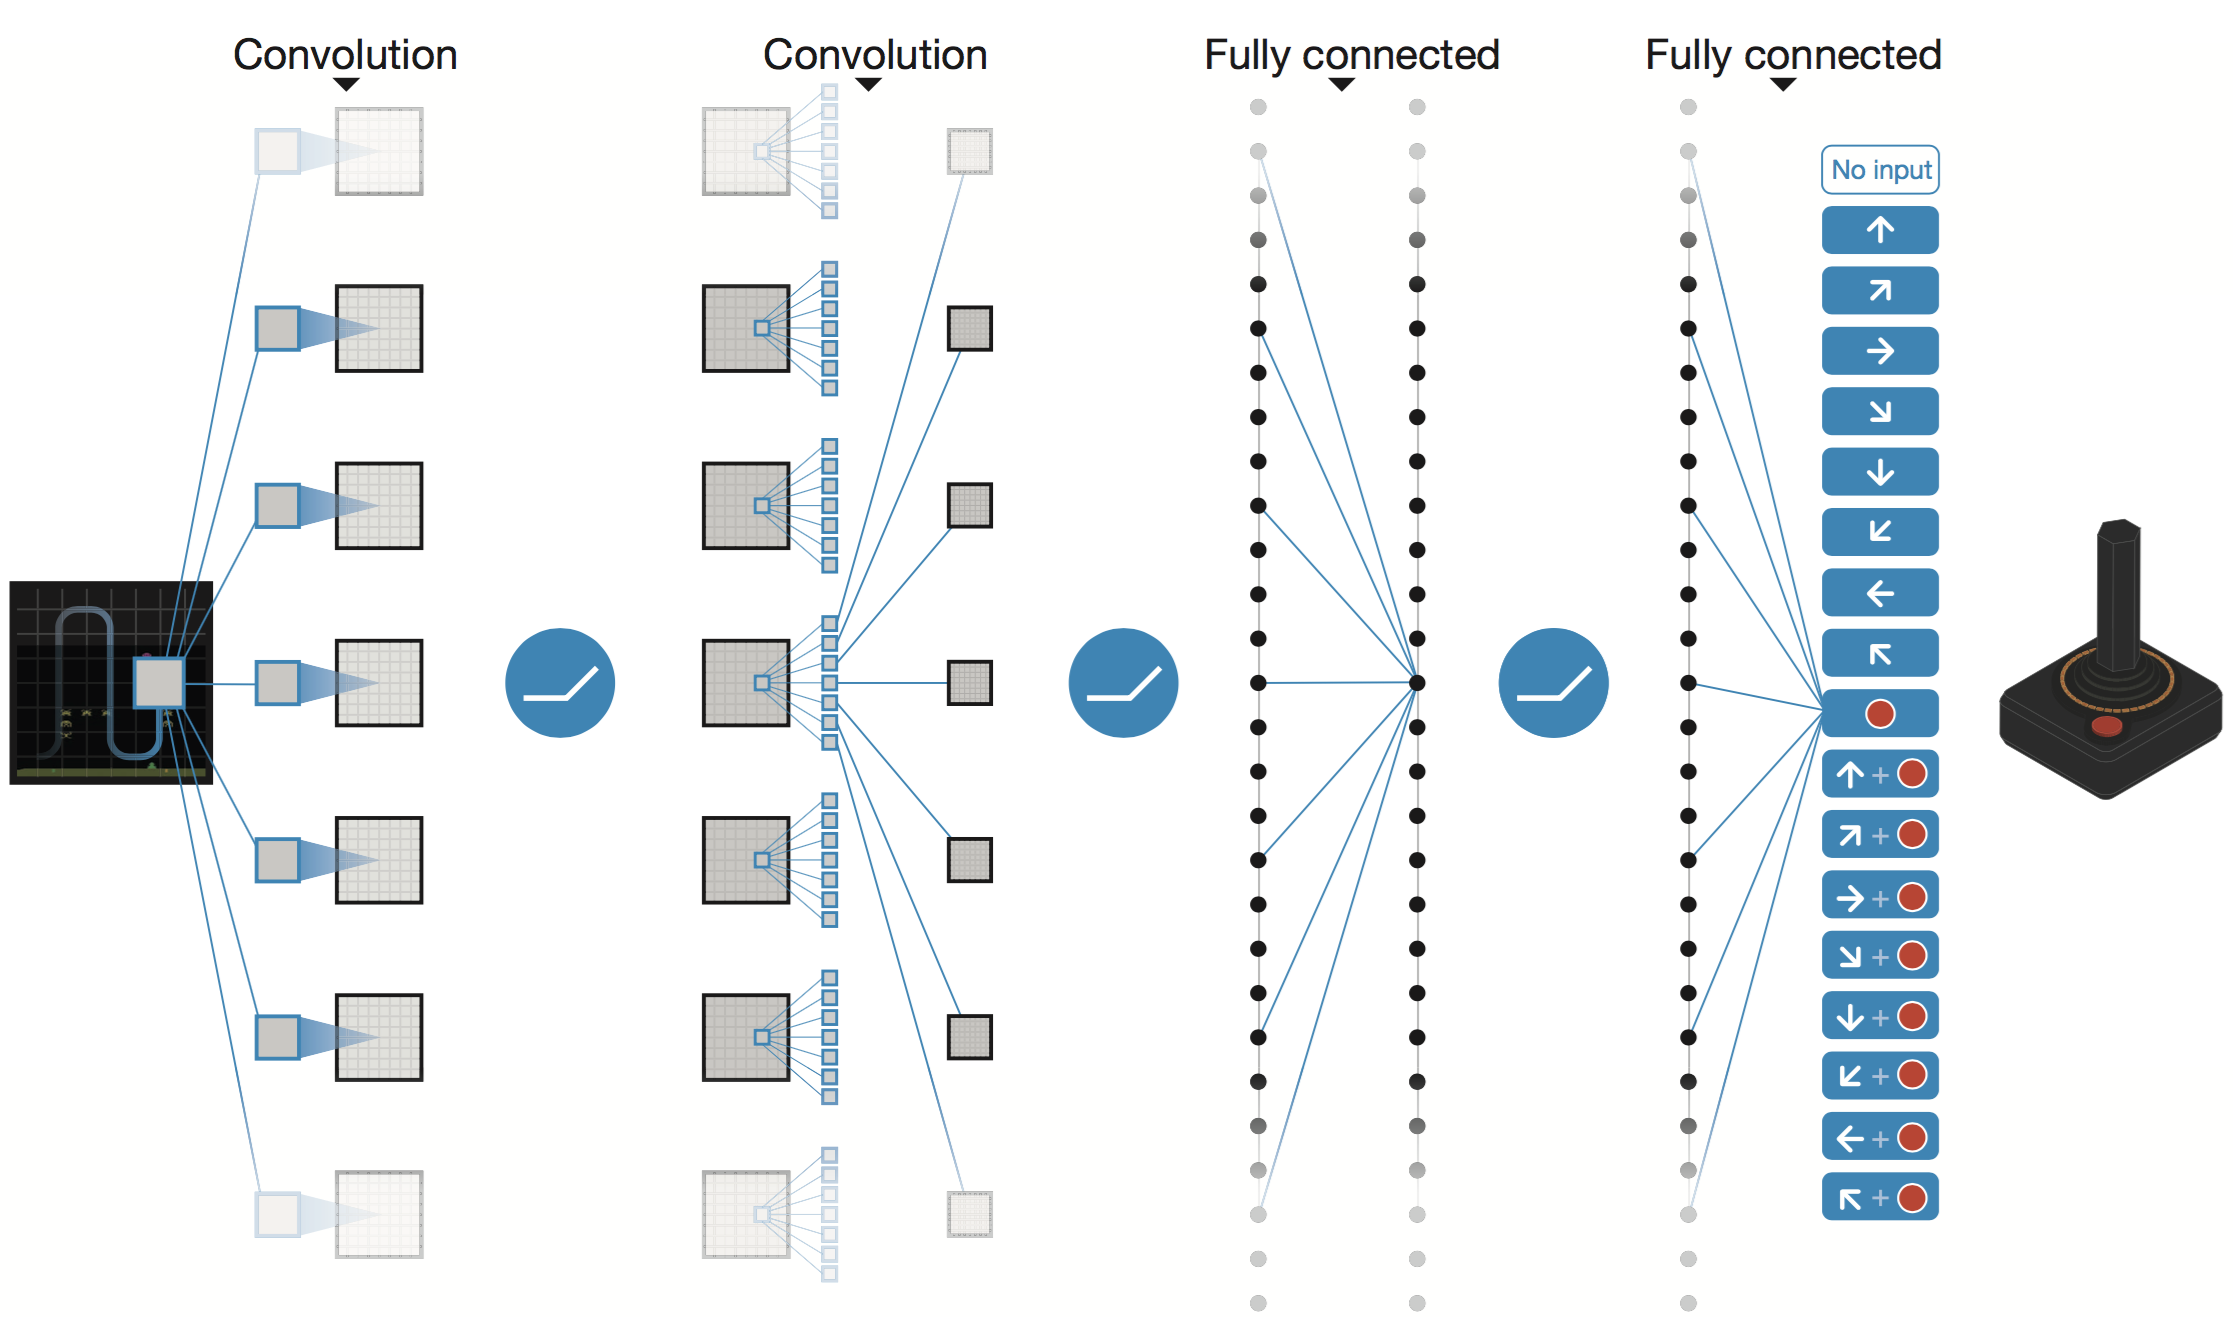
\includegraphics[width=1.0\textwidth]{CNN_DQN}
\caption{DQN状态行为值函数逼近网络}
\label{fig:CNN_DQN}
\end{figure}

我们知道,神经网络的训练是一个最优化过程,目的是让损失函数最小化,而损失函数是标签和网络输出的偏差。为此,我们需要巨量的带有标签的数据,然后通过反向传播使用梯度下降的方法来更新神经网络的参数。然而,强化学习只有奖赏的返回值,所以需要我们通过Q-learning算法使用奖赏为DQN网络提供带有标签的样本。

在算法$\ref{algo:algorithm_2}$中,我们知道Q目标是$R_{t+1}+\gamma \max_{a}(Q(S_{t+1},a))$,而我们学习Q值函数的目的就是趋近Q值目标值。因此,DQN网络训练的损失函数为:
\begin{equation}
\label{seq_3_2_1}
\begin{aligned}
L(\theta)=\mathbb{E}[(\underbrace{r+\gamma\max_{a^{'}} Q(s^{'},a^{'};\theta)}_{Target}-Q(s,a;\theta))^{2}]
\end{aligned}
\end{equation}
公式$\eqref{seq_3_2_1}$中,$s^{'}$,$a^{'}$分别表示下一个状态和行为。这里使用Q-learning要更新的Q值值函数作为目标值。有了目标值,又有当前值,那么偏差就能通过均方差来进行计算。接着我们可以按照第二章参数化函数逼近的训练步骤,先求出损失函数的梯度,然后利用随机梯度下降法(Stochastic Gradient Descent, SGD)来更新参数,从而得到最优的Q值函数。

其实,早在1995年Bertsekas等人就将神经网络应用在在强化学习的值函数逼近中,取得了相比线性逼近较好的结果,但是往往会出现不稳定不收敛的情况\citep{bertsekas1995neuro}。此后,众多学者在这个方向上一直没有突破,直到DeepMind团队的出现。

 \paragraph{设置经验回放机制}
DeepMind团队的创始人Hassabis是神经科学的博士,他主要研究人类大脑中的海马体,海马体是大脑中主要负责记忆和学习的部分。他在研究时发现,人类在睡觉的时候,海马体会把一天的记忆重放给大脑皮层,利用这个启发机制,DeepMind团队的研究人员设计了一种神经网络的训练方法:经验回放。

如图$\ref{fig:experience_reply}$所示,经验回放是将探索环境得到的转移样本($s_{t}, a_{t}, r_{t+1}, s_{t+1}$)存储在一个数据库(回放记忆单元)中,再利用随机均匀采样的方法从数据库中抽取转移样本,训练神经网络。在训练神经网络时,我们假设训练数据是独立同分布的,但是通过强化学习采集的数据之间存在关联性,利用这些数据进行顺序训练,神经网络难免会不稳定。利用经验回放可以打破这种数据间的关联性,从而解决了数据相关性以及数据的非静态分布的问题,使的神经网络训练收敛且稳定。
\begin{figure}[htbp]
\centering
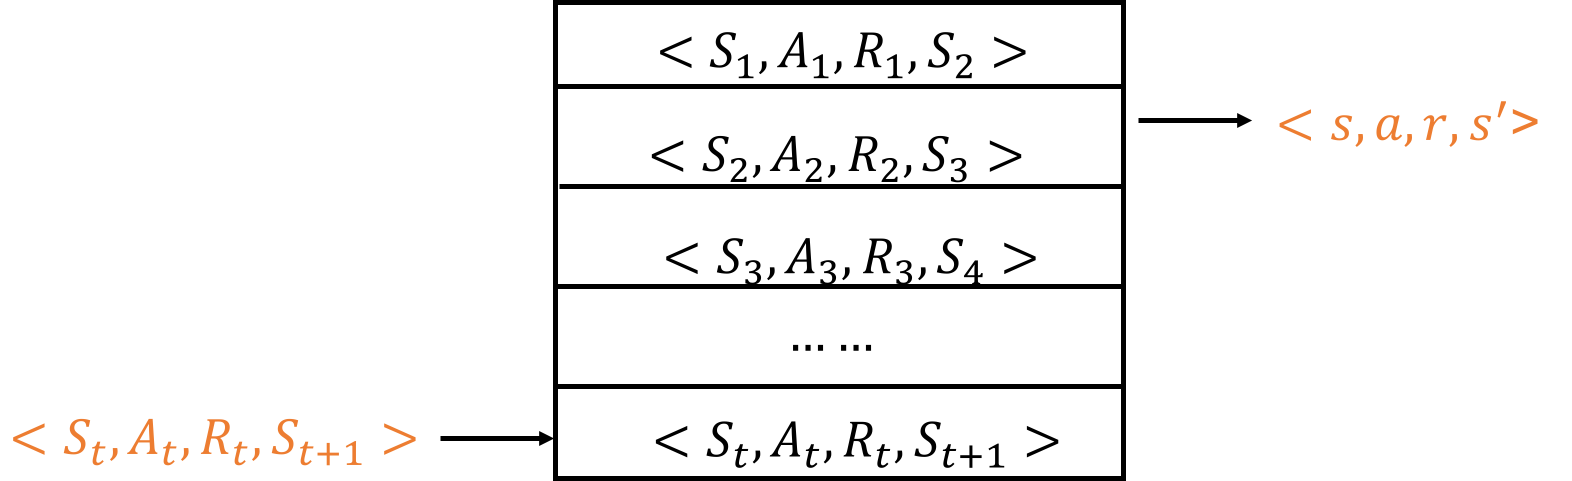
\includegraphics[width=1.0\textwidth]{experience_reply}
\caption{经验回放机制}
\label{fig:experience_reply}
\end{figure}

 \paragraph{设置独立的目标网络}
从上面的分析中,我们知道DQN使用了梯度下降法对参数$\mathbf{\theta}$进行更新:
\begin{equation}
\begin{aligned}
\mathbf{\theta}_{t+1}=\mathbf{\theta}_{t}+\alpha[\underbrace{r+\gamma \max_{s^{'}}Q(s^{'},a^{'};\mathbf{\theta})}_{Target}-Q(s,a;\mathbf{\theta})]\triangledown Q(s,a;\mathbf{\theta})
\end{aligned}
\end{equation}
其中,$r+\gamma \max_{s^{'}}Q(s^{'},a^{'};\mathbf{\theta})$为Q目标值,在计算$\max_{s^{'}}Q(s^{'},a^{'};\mathbf{\theta})$时用到的参数向量为$\mathbf{\theta}$。

在DQN算法出现之前,利用神经网络逼近值函数时,计算Q目标所用的网络参数向量为$\mathbf{\theta}$,与梯度计算时所用的参数向量相同,这样就容易导致数据间存在关联性,从而使训练不稳定。为了解决此问题,DeepMind提出使用另一个目标网络(TargetNet)产生Q目标值。具体地,$\mathbf{\theta}$代表当前网络(MainNet)的输出,用来评估当前状态行为对的值函数;$\mathbf{\theta}^{-}$代表目标网络的输出,依此求出Q目标值。并且,用于状态行为值函数逼近的网络每一步都要更新,而用于计算目标的网络则是每个固定的步骤更新一次。

因此,值函数的更新变为:
\begin{equation}
\begin{aligned}
\mathbf{\theta}_{t+1}=\mathbf{\theta}_{t}+\alpha[\underbrace{r+\gamma \max_{s^{'}}Q(s^{'},a^{'};\mathbf{\theta^{-}})}_{TargetNet}-\underbrace{Q(s,a;\mathbf{\theta})]\triangledown Q(s,a;\mathbf{\theta})}_{MainNet}
\end{aligned}
\end{equation}

 \paragraph{DQN框架}
 至此,在Q-learning算法的基础上并经过以上三个方面的改进,就可以得到DQN的算法流程图$\ref{fig:liuchengtu_DQN}$。从图中可以看出,,DQN的主要学习过程包括以下几步:
\begin{figure}[htbp]
\centering
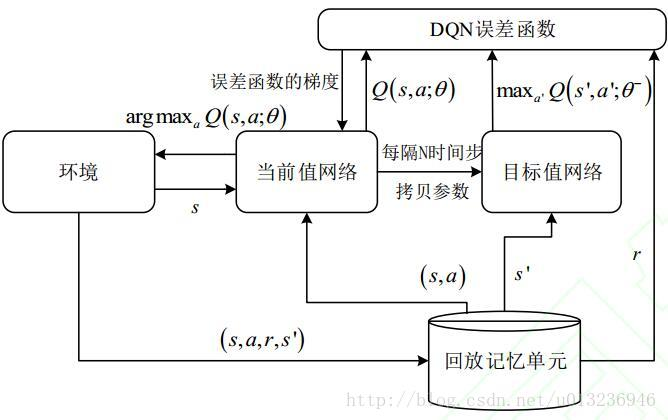
\includegraphics[width=0.9\textwidth]{liuchengtu_DQN}
\caption{DQN流程图}
\label{fig:liuchengtu_DQN}
\end{figure}

(1)构建回放记忆单元。在每个情节中,首先初始化第一个状态$s$,并在接下来的每个时间点,按照$\epsilon-greedy$策略选择行为$a$,并在仿真器中执行,即可得到对应的即时奖赏$r$和下一步的状态$s^{'}$。并将此转换样本($s,a,r,s^{'}$)放到回放记忆单元中。

(2)值函数的学习。从回放记忆单元中随机选取一条转移样本($s,a,r,s^{'}$),并分别使用当前值网络MainNet和目标值网络TargetNet分别计算出值函数的估计值 $Q(s,a;\mathbf{\theta})$和Q目标值$r+\gamma \max_{s^{'}}Q(s^{'},a^{'};\mathbf{\theta^{-}})$,然后计算误差函数$L=(r+\gamma \max_{s^{'}}Q(s^{'},a^{'};\mathbf{\theta^{-}})-Q(s,a;\mathbf{\theta}))^{2}$,并使用梯度下降法进行求解。损失函数的构建过程参见图$\ref{fig:loss_DQN}$

(3)更新目标网络参数。经过若干步的训练后,将当前网络的参数拷贝给目标网络,进行目标网络的参数更新。

% 在DQN中增强学习Q-Learning算法和深度学习的SGD训练是同步进行的

\begin{figure}[htbp]
\centering
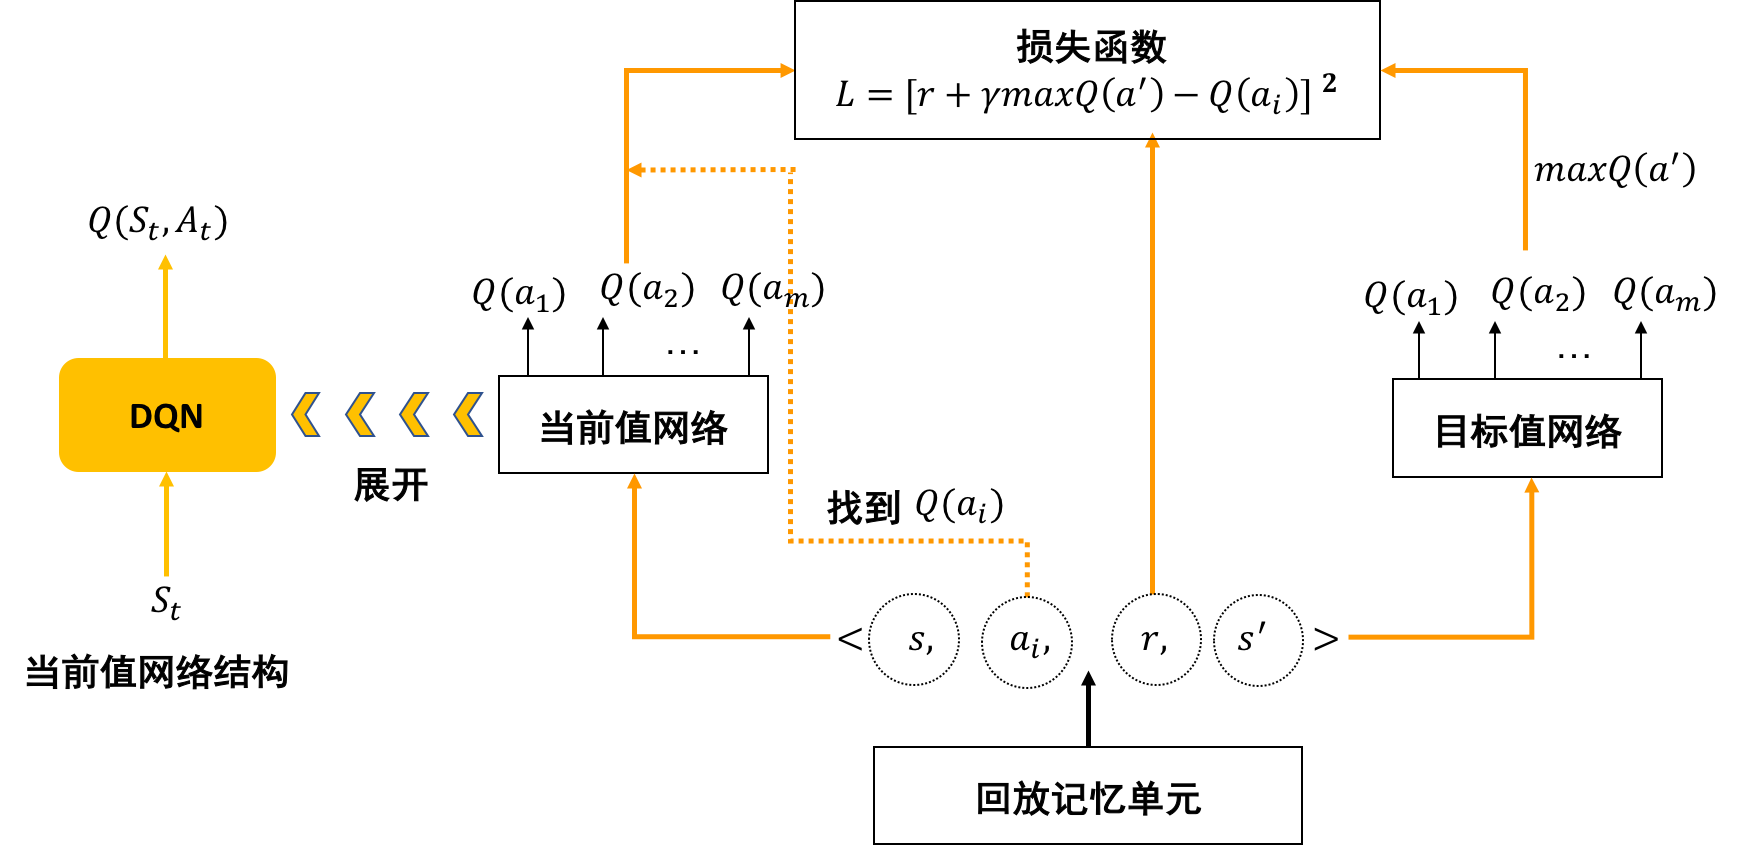
\includegraphics[width=0.8\textwidth]{loss_DQN}
\caption{DQN损失函数构造}
\label{fig:loss_DQN}
\end{figure}

综合考虑以上所有的内容,可以得到DQN的伪代码如算法$\ref{algo:algorithm_DQN}$所示。

\begin{algorithm}[htbp]
\small
\SetAlgoLined
\SetKwRepeat{Repeat}{repeat}{until} 
初始化回放记忆库$D$,记忆库大小为$N$\;
利用随机权值$\mathbf{\theta}$初始化状态行为值函数$Q$\;
初始化$\mathbf{\theta}^{-}$,令$\mathbf{\theta}^{-}=\mathbf{\theta}$,用以计算Q目标值\;
\For{$episode=1,\cdots, M$}{
	初始化情节的第一个状态:$s_{1}={x_{1}}$(${x_{1}}$为环境的观测特征),通过预处理得到该状态对应的特征输入:$\phi_{1}=\phi(s_{1})$\;
	\For{$t=1,\cdots, T$}{
		以概率$\epsilon$选一个随机行为$a_{t}$\;
		如果以上小概率事件没有发生,则按照贪婪策略选择当前值函数最大的那个行为:$a_{t}=\argmax_{a}Q(\phi(s_{t}),a;\mathbf{\theta})$\;
		在仿真器中执行行为$a_{t}$,可以得到奖赏$r_{t+1}$以及环境的下一步观测特征$x_{t+1}$\;
		设置$s_{t+1}=s_{t},a_{t},x_{t+1}$,预处理得到对应的特征输入:$\phi_{t+1}=\phi(s_{t+1})$\;
		将转换样本($\phi_{t}, a_{t}, r_{t}, \phi(s_{t+1})$)放到回放记忆库中\;
		从回放记忆库D中均匀随机采样一小批转换样本($\phi_{j}, a_{j}, r_{j+1}, \phi(s_{j+1})$)\;
		判断是否是一个情节的终止状态,若是,则Q目标值为$r_{j+1}$,否则利用Q目标网络$\mathbf{\theta}^{-}$计算Q目标$r_{j+1}+\gamma \max_{s^{'}}Q(s^{'},a^{'};\mathbf{\theta^{-}})$\;
		使用随机梯度下降算法更新当前网络参数:$\triangle \theta = \alpha [r+\gamma \max_{a^{'}}Q(s^{'},a^{'};\theta^{-})-Q(s,a;\theta) ]\triangledown_{Q}(s,a;\mathbf{\theta})$\;
		更新状态行为值函数逼近的网络参数:$\mathbf{\theta}=\mathbf{\theta}+\triangle \theta$\;
		每隔$C$步更新一次Q目标网络权值;即:$\mathbf{\theta}^{-}=\mathbf{\theta}$\;
	}
}
% 输出最终策略:$\pi(s)=\argmax_{a}Q(s,a)$\;
\caption{DQN伪代码}
\label{algo:algorithm_DQN}
\end{algorithm}

\subsection{基于DQN的基准模型}
我们可以直接将DQN模型用于直接营销的场景中。具体做法就是将客户的观测值作为状态$s$,企业得到的利润作为即时奖赏$r$,是否采取营销作为行为$a$,然后按照上述DQN(算法$\ref{algo:algorithm_DQN}$)的方式去训练网络的参数以得到一个近似Q函数。经过若干循环的训练,当得到一个很好的Q函数后,我们就可以按照贪婪的方式从中选择行为$\pi(s):=\argmax_{a}Q(s,a)$。

与算法$\ref{algo:algorithm_DQN}$不同的是,我们不需要通过与模拟器的进行交互而产生训练数据,而是通过对原始数据样本进行处理,形成($s_{t},a_{t},r_{t},s_{t+1}$)的形式的初始化记忆库。
% 另外,在从初始化记忆库中随机抽取minibatch个状态的时候,我们的所使用的方法是minibatch不应该很大,而且minibatch

图$\ref{fig:dqn_crm}$为DQN的网络结构。可以看出,前一个输入和后一个输入之间是没有关系的。其中,$o_{t}$为观测值,$\tilde{h}_{t}$为CNN的隐状态,$Q(s_{t},a_{t})$为在$t$时刻时,执行行为$a$所的到的Q估计值。

\begin{figure}[htbp]
\centering
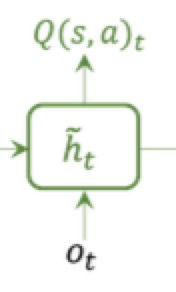
\includegraphics[width=0.2\textwidth]{dqn_crm}
\caption{DQN}
\label{fig:dqn_crm}
\end{figure}

\section{基于RNN的深度强化学习混合模型}
因为卷积神经网络无法对时间序列上的变化进行建模,所以本章考虑使用循环神经网络(Recuurent Neural Network, RNN)以及它的改进版本长短时记忆网络(Long  Short-Term Memory,LSTM),并详细介绍了这两种神经网络在解决序列问题上的优势,然后在此基础上提出了基于RNN的深度强化学习混合模型:独立两网络模型RNN+DQN、一步混合模型1-RNN+DQN和两步混合模型2-RNN+DQN。

\subsection{RNN和LSTM}
在DQN中,逼近Q值函数时所使用网络结构是卷积神经网络CNN,它的结构有一个特点:假设输入是一个独立的没有上下文联系的单位,即前一个输入和后一个输入是没有关系的,所以CNN无法对时间序列上的变化进行建模。但是,像直复营销这种序列决策的应用场景中,前面的输入和后面的输入肯定是有关系的,这时就需要用到深度神经网络中的另外一个利器,循环神经网络,它可以很好处理这种时间序列上的变化。因此,在神经网络结构的选择上,本章考虑使用循环神经网络RNN以及它的改进版本长短时记忆网络LSTM。

 \paragraph{RNN}
RNN是一种对序列数据建模的神经网络,可以连接先前的信息到当前的任务上来。具体的做法是:网络会对前面的信息进行记忆存储并应用于当前输出的计算中,即隐藏层之间的节点不再无连接而是有连接的,并且隐藏层的输入不仅包括输入层的输出还包括上一时刻隐藏层的输出。图$\ref{fig:rnn}$是一个RNN模型的简化结构展开图。
\begin{figure}[htbp]
\centering
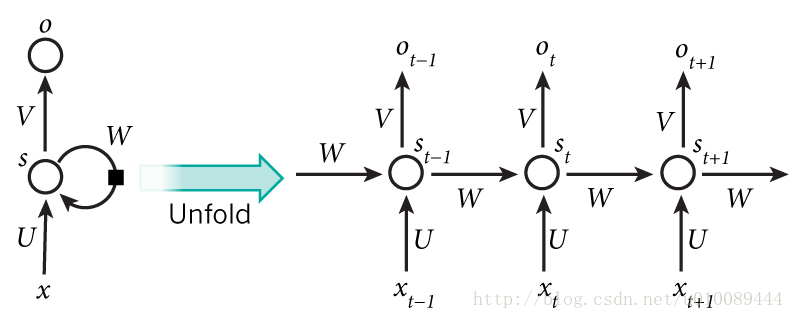
\includegraphics[width=0.8\textwidth]{rnn}
\caption{RNN模型的简化结构展开图}
\label{fig:rnn}
\end{figure}

在图$\ref{fig:rnn}$中:$x_{t}$表示$t$时刻的输入;$s_{t}$表示$t$时刻的隐藏层的值(memory),它基于上一时刻的隐状态和当前输入得到:$s_t=f(U x_{t}+W s_{t−1})$,其中$f(\cdot)$一般是非线性的激活函数;
% 在计算$s_{0}$时,即第一个单词的隐藏层状态,需要用到$s_{−1}$,但是其并不存在,在实现中一般置为0。
$o_{t}$表示$t$时刻的输出。$U$是输入层到隐藏层的权重矩阵,$V$是隐藏层到输出层的权重矩阵,权重矩阵$W$就是隐藏层上一次的值作为这一次的输入的权重。需要注意的是:在传统神经网络中,每一个网络层的参数是不共享的,而在RNN中,所有层次均共享同样的参数,
% 其反应出RNN中的每一步都在做相同的事,只是输入不同,
因此大大地降低了网络中需要学习的参数。

网络在$t$时刻接收到输入$x_{t}$之后,隐藏层的值是$s_{t}$,输出的值是$o_{t}$。
% 特别的,$o_{t}$的值不仅仅取决于$x_{t}$,还取决于$o_{t-1}$。
我们可以用下面的公式来表示循环神经网络的计算方法:
\begin{equation}
\label{rnn_1}
\begin{aligned}
o_{t}=g(V s_{t})
\end{aligned}
\end{equation}
\begin{equation}
\label{rnn_2}
\begin{aligned}
s_{t}=f(U x_{t}+W s_{t-1})
\end{aligned}
\end{equation}
式\eqref{rnn_1}是输出层的计算公式,输出层是一个全连接层,也就是它的每个节点都和隐藏层的每个节点相连。$V$是输出层的权重矩阵,$g$是激活函数。式\eqref{rnn_2}是隐藏层的计算公式,它是循环层。$U$是输入$x$的权重矩阵,$W$是上一次的值作为这一次的输入的权重矩阵,$f$是激活函数。从上面的公式我们可以看出,循环层和全连接层的区别就是循环层多了一个权重矩阵$W$。如果反复把式$\eqref{rnn_2}$带入到式$\eqref{rnn_1}$,我们将得到:
\begin{equation}
\label{rnn_3}
\begin{aligned}
o_{t}&=g(V s_{t})\\
&=V f(U x_{t}+W s_{t-1})\\
&=V f(U x_{t}+W f(U x_{t-1}+W s_{t-2}))\\
&=V f(U x_{t}+W f(U x_{t-1}+W f(U x_{t-2}+W f(U x_{t-3}+\cdots)))\\
\end{aligned}
\end{equation}

从式\eqref{rnn_3}可以看出,循环神经网络的输出值$o_{t}$,是受前面历次输入值$x_{t}$、$x_{t-1}$、$x_{t-2}$、$x_{t-3}$、$\cdots$影响的,这就是为什么循环神经网络可以往前看任意多个输入值的原因。

RNN的训练方法是采用基于时间的反向传播算法(BackPropagation Through Time, BPTT),具体的更新方法和BP更新方法相同。但是,在处理较长序列的时候, RNN不能得到较好的性能。一个主要原因是,RNN在训练中如果向前考虑的很远的时候,会导致对应的误差项的值增长或者缩小的非常快,就会很容易发生梯度爆照或者梯度消失的现象,这导致训练时梯度不能在较长序列中一直传递下去,从而使RNN无法捕捉到长时间距离的影响。由此,提出了长短时记忆网络LTSM。

% 通常来说,梯度爆炸更容易处理一些。因为梯度爆炸的时候,我们的程序会收到NaN错误。我们也可以设置一个梯度阈值,当梯度超过这个阈值的时候可以直接截取。梯度消失更难检测,而且也更难处理一些,除了合理的初始化权重值、使用relu代替sigmoid和tanh作为激活函数外,还可以使用其他诸如的方法。其中后者是目前最流行的方法。

 \paragraph{LSTM}
% 在该部分中,我们通过简要的介绍LSTM的原理,来了解LSTM可以解决长距离依赖问题的原因。
因为原始RNN的隐藏层只有一个状态,它对于短期的输入非常敏感,LSTM在此基础上增加了一个状态,让它保存长期的状态,从而解决了传统RNN无法处理长距离依赖的问题。新增加的状态称为单元状态(Cell State)。

如图$\ref{fig:lstm_2}$所示为LSTM按时间维度的展开结构图,灰色矩形部分代表一个LSTM的结构,其中h为原始RNN的隐藏层状态,c为单元状态。从图中我们可以看出,在t时刻,LSTM的输入有三个:当前时刻网络的输入值$x_{t}$、上一时刻LSTM的输出值$h_{t-1}$、以及上一时刻的单元状态$c_{t-1}$;同时,LSTM的输出有两个:当前时刻LSTM输出值$h_{t}$、和当前时刻的单元状态$c_{t}$。
% 注意$x$、$h$、$c$都是向量。

\begin{figure}[htbp]
\centering
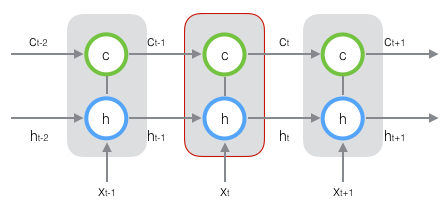
\includegraphics[width=0.8\textwidth]{lstm_2}
\caption{LSTM按时间维度展开图}
\label{fig:lstm_2}
\end{figure}

LSTM提出使用三个控制开关来控制长期单元状态c。第一个开关,负责控制继续保存长期状态c;第二个开关,负责控制把即时状态输入到长期状态c;第三个开关,负责控制是否把长期状态c作为当前的LSTM的输出。上述表述的开关在LSTM中使用的门(gate)来实现的,门实际上就是一层全连接层,它的输入是一个向量,输出是一个0到1之间的实数向量。假设$W$是门的权重向量,$b$是偏置项,那么门可以表示为:
\begin{displaymath}
\begin{aligned}
g(x)=\sigma (W x+b)
\end{aligned}
\end{displaymath}

门的使用,就是用门的输出向量按元素乘以我们需要控制的那个向量。因为门的输出是0到1之间的实数向量,那么,当门输出为0时,任何向量与之相乘都会得到0向量,这就相当于啥都不能通过;输出为1时,任何向量与之相乘都不会有任何改变,这就相当于啥都可以通过。因为$\sigma$(也就是sigmoid函数)的值域是(0,1),所以门的状态都是半开半闭的。

图$\ref{fig:lstm}$所示为LSTM的内部结构。LSTM用两个门来控制单元状态c的内容,一个是遗忘门(Forget Gate),它决定了上一时刻的单元状态$c_{t-1}$有多少保留到当前时刻;另一个是输入门(Input Gate),它决定了当前时刻网络的输入$x_{t}$有多少保存到单元状态。另外,LSTM用输出门(Output Gate)来控制单元状态$c_{t}$有多少输出到LSTM的当前输出值$h_{t}$。

其中,遗忘门可表示为:
\begin{equation}
\label{lstm_1}
\begin{aligned}
f_{t}=\sigma (W_{f} \cdot [h_{t-1}, x_{t}]+b_{f})
\end{aligned}
\end{equation}
在式\eqref{lstm_1}中,$W_{f}$ 是遗忘门的权重矩阵,$[h_{t-1}, x_{t}]$表示把两个向量连接成一个更长的向量,$b_{f}$是遗忘门的偏置项,$\sigma$是sigmoid函数。

输入门可表示为:
\begin{equation}
\label{lstm_2}
\begin{aligned}
i_{t}=\sigma (W_{i} \cdot [h_{t-1}, x_{t}]+b_{i})
\end{aligned}
\end{equation}
在式\eqref{lstm_2}中,$W_{i}$是输入门的权重矩阵,$b_{i}$是输入门的偏置项。

然后,根据上一次的输出和本次输入,来计算用于描述当前输入的单元状态$\tilde{c}_{t}$:
\begin{equation}
\label{lstm_3}
\begin{aligned}
\tilde{c}_{t}=\tanh (W_{c} \cdot [h_{t-1}, x_{t}]+b_{c})
\end{aligned}
\end{equation}

接着,计算当前时刻的单元状态$c_{t}$:
\begin{equation}
\label{lstm_4}
\begin{aligned}
c_{t}=f_{t} \circ c_{t-1} + i_{t} \circ \tilde{c}_{t}
\end{aligned}
\end{equation}
式\eqref{lstm_4}中,符号$\circ$表示按元素乘。它是由上一次的单元状态$c_{t-1}$按元素乘以遗忘门$f_{t}$,再用当前输入的单元状态$\tilde{c}_{t}$按元素乘以输入门$i_{t}$,再将两个积加和产生的。我们就把LSTM关于当前的记忆$\tilde{c}_{t}$和长期的记忆$c_{t-1}$组合在一起,形成了新的单元状态$c_{t}$。

输出门,它控制了长期记忆对当前输出的影响:
\begin{equation}
\begin{aligned}
o_{t}=\sigma(W_{\sigma} \cdot [h_{t-1}, x_{t}]+b_{o})
\end{aligned}
\end{equation}

LSTM最终的输出,是由输出门和单元状态共同确定的:
\begin{equation}
\begin{aligned}
h_{t}=o_{t} \circ \tanh(c_{t})
\end{aligned}
\end{equation}

\begin{figure}[htbp]
\centering
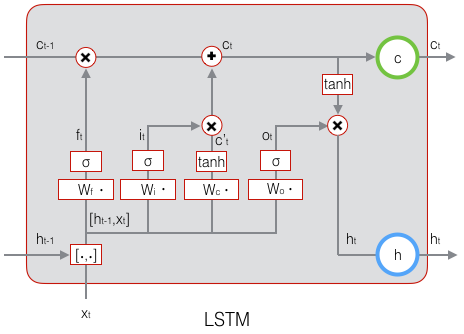
\includegraphics[width=0.8\textwidth]{lstm}
\caption{LSTM内部结构}
\label{fig:lstm}
\end{figure}

以上就是LSTM的前向计算。关于LSTM的训练过程仍然采用的反向传播算法,因为篇幅的限制具体计算过程不详细展开。综上所述,我们可以看到,在LSTM中,由于遗忘门的控制,它可以保存很久很久之前的信息,由于输入门的控制,它又可以避免当前无关紧要的内容进入记忆,这两部分的相互配合使得LSTM可以较好的处理长时间依赖的问题。

% 主要包括以下三步:

% (1)前向计算每个神经元的输出值,对于LSTM来说,即 $\mathbf{f}_{t}$、$\mathbf{i}_{t}$、$\mathbf{c}_{t}$、$\mathbf{o}_{t}$、$\mathbf{h}_{t}$五个向量的值。。

% (2)反向计算每个神经元的误差项值。与循环神经网络一样,LSTM误差项的反向传播也是包括两个方向:一个是沿时间的反向传播,即从当前t时刻开始,计算每个时刻的误差项;一个是将误差项向上一层传播。

% (3)根据相应的误差项,计算每个权重的梯度。

 \paragraph{基于RNN和LSTM的基准模型}
 作为对照的基准模型,我们考虑仅使用RNN模型或者LSTM模型来解决直接营销的问题,那么,此问题就被看作是一个监督学习问题。

 在监督学习的过程中,需要有特征和标签。这我们的实验中,特征就是客户每一时刻的状态和企业是否进行了营销这一行为所组成的向量,标签就是企业所得到的即时利润。如图$\ref{fig:rnn_}$所示为RNN的学习过程,将每个客户的交互历史看成一个序列。训练阶段,在时刻$t$时,需要将观测$o_{t}$,奖赏$r_{t}$和隐藏状态$\tilde{h}_{t-1}$带入RNN网络,然后使用真实的奖赏与预测的奖赏之间的均方误差作为损失函数训练更新模型。测试阶段,训练完成后的模型记作$\hat{R}$,将此时的观测值$o_{t}$和上一时刻的隐藏状态$\tilde{h}_{t-1}$作为输入,带入模型$\hat{R}$,然后再以贪婪的方式选择每个客户的合适营销行为:$\argmax_{a}\hat{R}(s,\tilde{h},a)$。LSTM与RNN的训练过程相同。

 但是,需要注意的是,与强化学习追求累积奖赏最大化不同,我们使用的监督学习只可以最大化即时奖赏。

\begin{figure}[htbp]
\centering
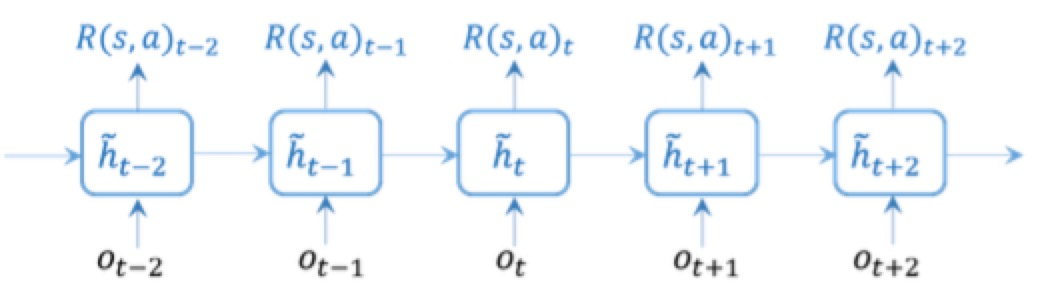
\includegraphics[width=1.0\textwidth]{rnn_}
\caption{rnn训练展开图}
\label{fig:rnn_}
\end{figure}

\paragraph{基于DRL(RNN)基准模型}
通过上述的分析我们知道,RNN和LSTM模型通过从历史数据中对未来奖赏的长期依赖性进行建模,可以捕捉到系统的复杂特征,进而可以较好的处理部分可观测的问题。而强化学习在处理序列决策时是以最大化累积奖赏为目标的,而不像监督学习那种仅仅追求即时奖赏最大化。如果将两个算法进行结合\citep{bakker2002reinforcement,hausknecht2015deep,lin1993reinforcement,narasimhan2015language},应用在序列化有关问题上,可以取得很好的表现。其中,在文献\citep{hausknecht2015deep,narasimhan2015language}中作者将DQN中的CNN网络换成RNN网络,应用在游戏、文本等场景,取得了比DQN更好的表现。

结合文献\citep{hausknecht2015deep,narasimhan2015language}所设计的模型,并且参考最新的DQN模型的处理技巧,我们设计了针对直接营销场景的模型DRL(RNN)作为第第三个对照基准试验。DRL(RNN)模型的结构图如$\ref{fig:rl_rnn}$所示,其中,$o_{t}$是观测值,$\tilde{h}_{t}$为RNN的隐藏状态,$Q(s,a)_{t}$是在$t$时刻,状态$s$为$\tilde{h}_{t}$时且采取行为$a$并且的预测Q值。

算法的流程大致和算法$\ref{algo:algorithm_DQN}$相同。不同的是不需要通过模拟器进行数据的采集,只需要将原始数据进行处理,形成回放记忆单元,另外,在函数逼近时,将CNN网络换成RNN网络。训练阶段,主要是学习关于当前观测$o_{t}$和隐藏状态$\tilde{h}_{t-1}$的Q值函数,并且随着时间的推移,隐藏状态的表示方法也在不断更新。在测试阶段,当Q值网络学习完毕后,以贪婪的方式选择最优的行为。

\begin{figure}[htbp]
\centering
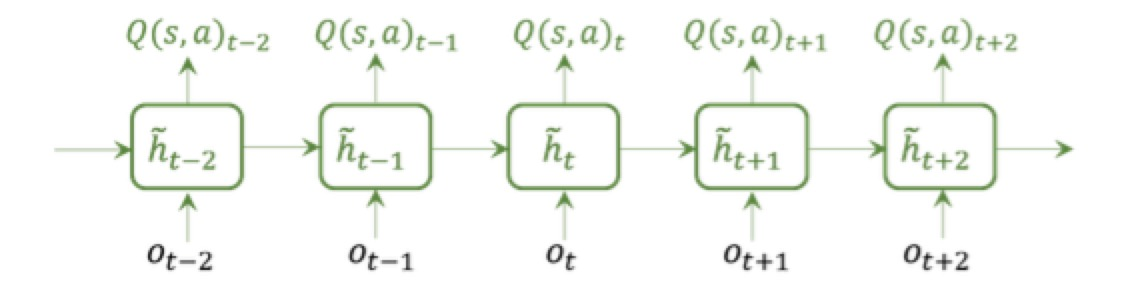
\includegraphics[width=1.0\textwidth]{rl_rnn}
\caption{RL-RNN框架}
\label{fig:rl_rnn}
\end{figure}

\subsection{两网络独立模型}
在DRL(RNN)模型中,循环神经网络起到两个作用,一方面,希望利用循环神经网络可以对序列的长时间依赖性进行建模的优势,以达到更好的解决部分可观测的问题,另一方面,循环神经网络最重要的作用是在强化学习的过程中进行Q值函数的逼近,然后利用评估的Q值函数通过贪婪的方式选择最优的行为。所以,在网络优化的过程中,我们需要同时兼顾对长期依赖性的学习和对最优策略的学习,这对于仅仅使用一个网络进行训练的模型来说是很难办到的。

受此启发,我们提出利用两个模型来解决上面的提出的问题。首先,使用一个RNN模型通过对长期依赖性进行建模,以更好的学习隐藏状态的表示方法;另外,使用DQN模型依靠其强大的非线性表达能力来逼近Q值函数,来进行最优策略的学习。第一个过程属于监督学习,可以充分发挥RNN序列建模的优势,第二个过程是强化学习过程,可以充分发挥其序列决策的优势,通过这种方法,使两个模型达到优势互补的目的。我们将此模型记为RNN+DQN、RNN+LSTM。

RNN+DQN模型的结构图如$\ref{fig:rnn+dqn}$所示。$o_{t}$是观测值,$h_{t}$是隐藏状态信息,$o_{t+1}^{'}$是$t+1$ 时刻的预测的观测值,$R_{t}$是预测的奖赏。训练阶段,先将所有数据的观测值带入到RNN模型,然后利用预测的下一状态值和即时奖赏值来训练RNN网络,当RNN训练结束后,再将数据的观测值带入RNN,并将RNN隐藏层状态作为DQN的输入,进行DQN网络的训练。测试阶段,利用上一时刻的隐状态和这一时刻的观测值作为RNN的输入,然后将产生的隐状态输入到已经学好的Q值网络中,以贪婪的方式选择最优的行为。

\begin{figure}[htbp]
\centering
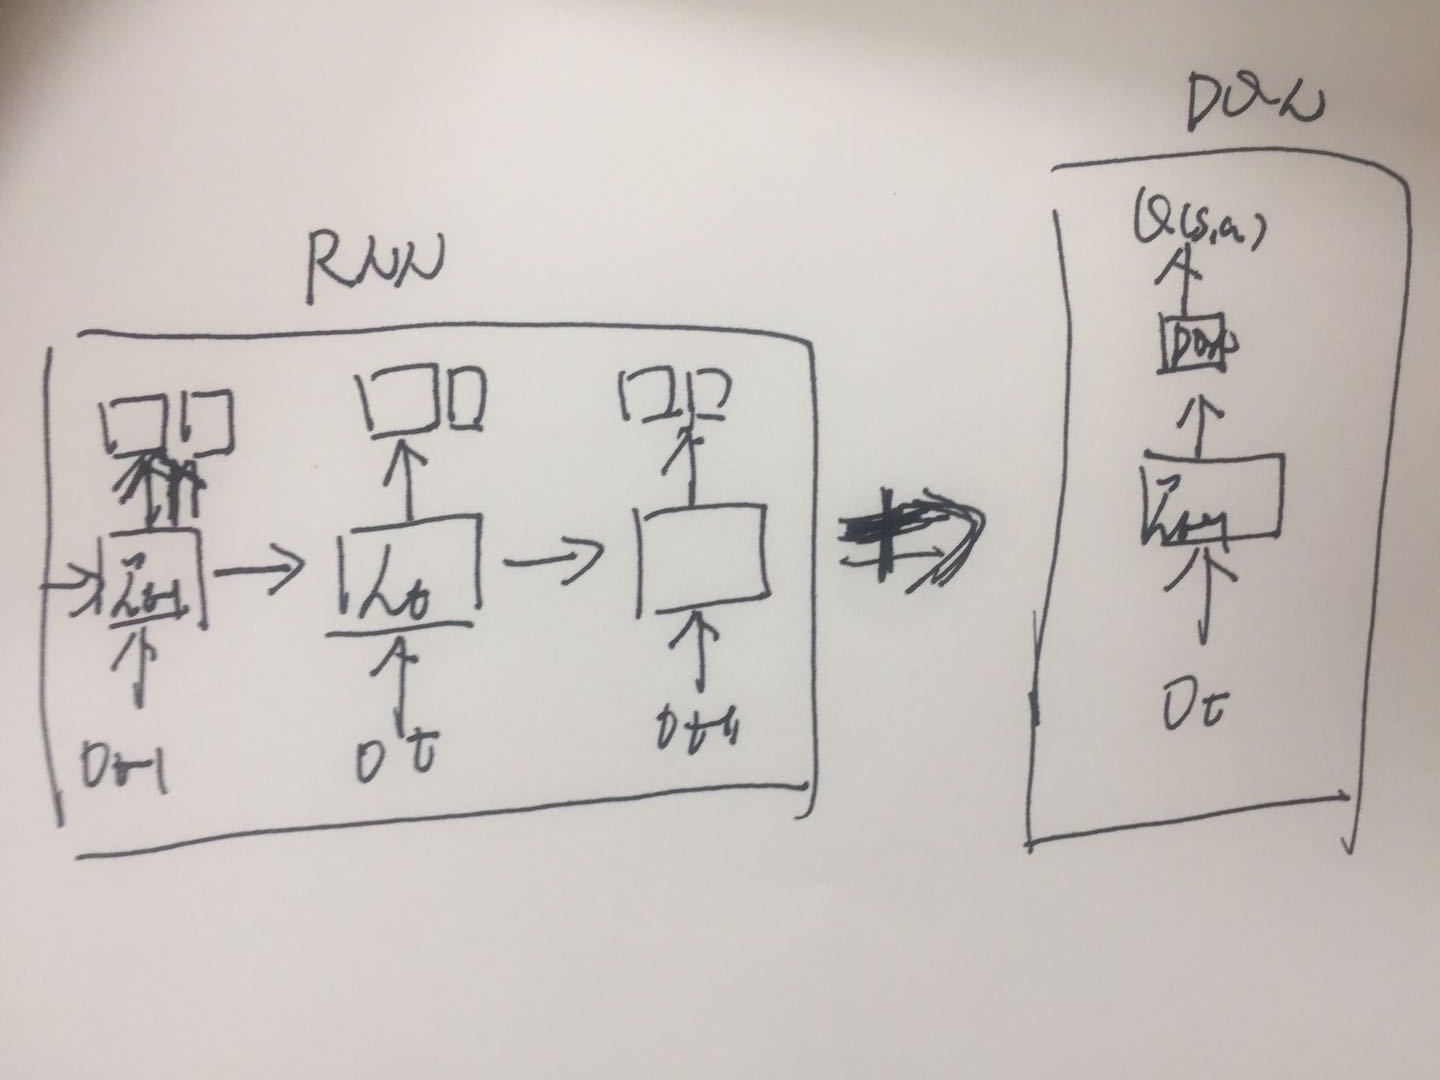
\includegraphics[width=0.8\textwidth]{rnn+dqn}
\caption{RNN+DQN框架}
\label{fig:rnn+dqn}
\end{figure}

\subsection{一步混合模型}
% 就像第一节所描述的那样,因为强化学习考虑到了未来的回报,而且它的目标是直接优化长期奖赏,这与在直复营销场景中所期望的最大化客户ltv的目标是一致的。
% 基于RNN的深度强化学习模型(RL-RNN和RL-LSTM)在模型的的计算和训练上与DQN是类似的,但是因为循环神经网络通过对未来奖赏的长短时依赖性进行建模从而可以更好的处理序列中的部分可观测问题的原因,被广泛应用在序列问题的处理上\citep{bakker2002reinforcement,hausknecht2015deep,lin1993reinforcement,narasimhan2015language}。它们所设计的模型可以使用图$\ref{fig:rl_rnn}$表示。

RNN+DQN模型虽然充分利用了两个不同类型的模型各自的优点,但是仍然存在以下问题。

1)训练过程比较复杂,需要等到RNN训练结束后,再将RNN训练好的信息代入DQN模型进行训练,在程序的实现上略显繁琐。

2)两个网络优化过程被完全割裂开来,这种方式会降低模型的鲁棒性。因为我们最终的目标是训练Q值网络,而在DQN的训练过程中,RNN网络是固定不变的,又因为在现实的场景中,环境的状态是在不断发生变化的,环境的表示方法也会发生一定的变化,或者说固定的神经网络结构只能在一定程度上捕捉到环境的隐藏信息,并不能一直捕捉到环境的隐藏信息。理想的情况是RNN在学到一个隐状态表法方式后就立刻让强化学习以此隐状态来最大化长期奖赏,两个网络在同时发生变化。

% 在RL-RNN模型中,因为RNN网络具有捕捉长期依赖性的强大能力,所以可以较好的估计Q函数。但是,在网络优化的过程中,RNN还需要可以很好的解决部分可观测的问题,那么如果要同时达到这两个目的,对于只有一个网络结构的RL-RNN来说是很难的。

所以,我们考虑具有两个网络的一步混合模型1-RNN-DQN。该网络结构如图$\ref{fig:rnn_dqn}$所示,其中,$o_{t}$是观测值,$h_{t}$是RNN的隐藏状态,$o_{t+1}^{'}$是$t+1$ 时刻预测的观测值,$R_{t}$是预测的即时奖赏,$Q(s,a)_{t}$是t时刻预测的Q值。蓝色部分对应着RNN网络的监督学习部分,红色部分对应着DQN的强化学习部分。同样地,在混合模型中,DQN的输入是RNN模型的隐状态。只不过在优化的过程中,两个部分一次交替进行。

训练阶段,使用联合训练的方法。首先,在每一个时刻,通过预测下一步的观测值和即时奖赏来训练RNN网络,然后将训练得到的环境的隐含信息作为DQN的输入,再通过DQN网络来逼近学习Q值函数。这两个训练步骤在随机梯度下降迭代过程中依此交替的进行。
可以看出,与文献\citep{hausknecht2015deep,narasimhan2015language}不同的是,在训练的过程中,监督信号将学习到的状态信息,反向传播到RNN的头部,而强化学习只是将误差信号反向传播到RNN隐藏层,不参加RNN的训练。
测试阶段,与RNN-DQN类似,将环境观测值输入RNN,然后将RNN的隐藏层信息作为状态导入到训练好的Q值网络中,以贪恋的方式选择最优行为。

因为在1-RNN-DQN学习的全部过程中,RNN和DQN模型按照上述训练方法依次,期间没有发生网络结构的变化,因此我们称之为一步混合模型,记为1-RNN-DQN。同样的方法,也可以得到1-LSTM-DQN。

% 可以使用强化学习模型,最大限度的获得长期回报,同时,可以对观测值和即刻奖赏的预测以训练优化监督学习模型,从而具有更好的推断和表示隐藏状态的能力。在这种混合方法中,使用监督学习来进行隐藏状态的表示学习,使用强化学习进行策略的学习,通过强化学习和监督学习的优势互补,可以使的这种混合模型达到很好的预测效果。另外,需要特别强调的是,这两个模型不能单独进行优化,而应该在监督学习了一个内部隐状态表示后就用强化学习模型最大化长期的奖赏。

% 使用以上混合模型的思想,我们可以得到基于rnn(lstm)和dqn的混合模型,即用rnn(lstm)进行监督模型的训练,使用dqn进行强化学习的训练,我可以将模型记为SL-RNN-RL-DQN(SL-LSTM-RL-DQN)。混合模型的网络结构如图$\ref{fig:rnn_dqn}$所示:

\begin{figure}[htbp]
\centering
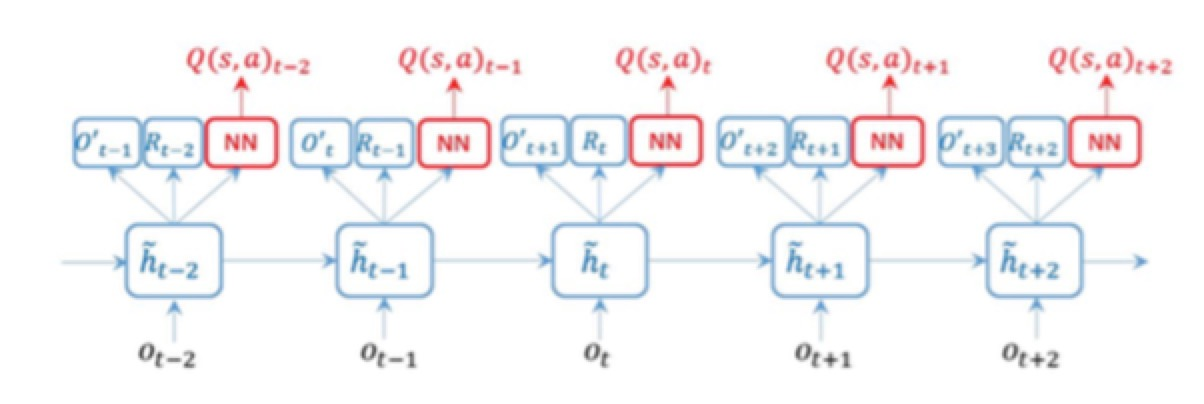
\includegraphics[width=1.0\textwidth]{rnn_dqn}
\caption{rnn-dqn框架}
\label{fig:rnn_dqn}
\end{figure}

% 在图$\ref{fig:rnn_dqn}$中,

% 由此,我们可以得到1-RNN-DQN模型的流程图以及损失函数的构造图。

\subsection{两步混合模型}
在1-RNN-DQN模型中,我们可以看到RNN网络和DQN网络之间并没有进行误差的传递,而是每个网络利用各自的误差进行计算。
% 在上述的1-RNN-DQN模型中,先使用监督模型rnn进行隐藏状态的表示学习,再使用dqn进行策略的学习。在训练的过程中,监督信号将学习到的状态信息,反向传播到rnn或者lstm的头部,而强化学习只是将误差信号反向传播到rnn隐藏层,不参加rnn的训练。
这种独立的误差计算方法虽然可以在一定程度上加快两个网络的训练速度,但是,因为两部分的误差信号是没有联系的,所以往往会因为这两个网络的训练不平衡性而影响了最终的预测性能。这种不平衡性主要表现在:

1)如果在某一时刻,经过之前的训练,RNN已经收敛,但是并不是全局收敛,而是局部收敛。这种情况下,会严重的影响DQN的训练效果。

2)我们最终的目标是为了训练Q值网络,而在1-RNN-DQN模型中,RNN的训练是和Q值没有必然联系的,从而割裂了两个网络整体的联系。

所以,基于以上的想法,我们提出了两步混合模型,记为2-RNN-DQN。如图$\ref{fig:2-rnn-dqn}$所示,2-RNN-DQN模型在训练时共分为两个阶段,第一阶段,按照1-RNN-DQN的方法进行训练,学习到两个网络的参数向量$\mathbf{\omega_{'}}$和$\mathbf{\omega_{''}}$,第二阶段,将RNN网络的隐藏层和DQN网络的输入层连接起来,组成一个新的网络结构$[\mathbf{\omega_{'}},\mathbf{\omega_{''}}]$,新的网络的输入是观测值,输出是Q函数。通过这种方式,便可以在第二阶段将Q值函数的误差反向传播到输入,从而提高学习的精度。策略决策时,直接利用第二阶段的整体网络进行测试,输出Q值函数,然后通过贪婪的方式选择最佳的行为。

需要注意的是,训练时两个阶段训练时间应该如何把握。本实验采用的方法是将训练数据集按照8:2的比例分成两份,第一份用于第一阶段的训练,第二份用于第二阶段的训练。同样的方法我们可以得到2-RNN-LSTM的模型。
% 具体学习过程是:将观测值输入到新的网络中,输出一个估计得Q值,然后利用误差学习更新整个网络的参数。

\begin{figure}[htbp]
\centering
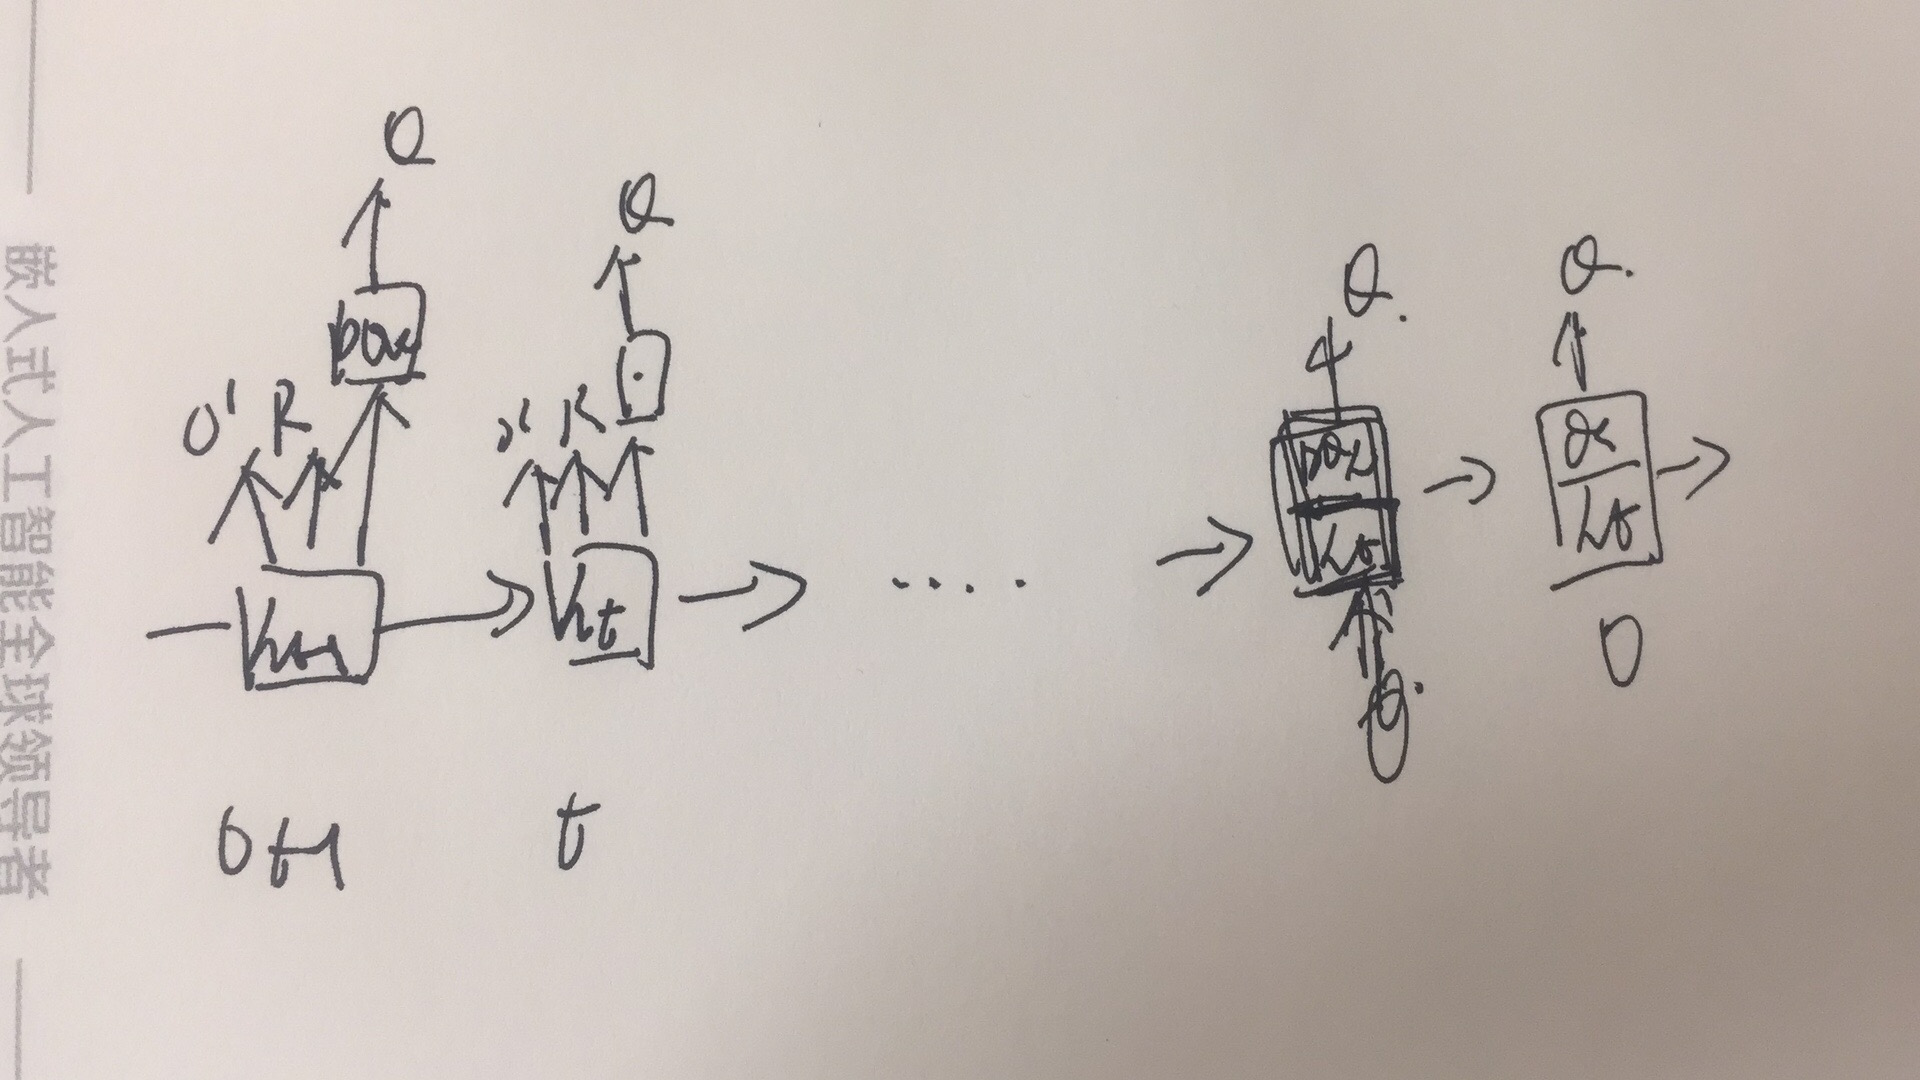
\includegraphics[width=1.0\textwidth]{2-rnn-dqn}
\caption{rnn-dqn框架}
\label{fig:2-rnn-dqn}
\end{figure}

% \subsection{对照实验模型}

% 到目前为止,我们已经得到了DQN、RL-RNN、RL-lstm、1-SL-RNN+RL-dqn、1-SL-lstm+RL-dqn、2-SL-RNN+RL-dqn、2-SL-lstm+RL-dqn的模型的方法,作为对照组,我们提供了监督学习的训练方法。

% 在监督学习的模型中,我们的目标是从给定的到目前为止的交互历史中,预测可以导致更高的即刻奖赏的行为。在我们的实验中,我们使用原始奖赏信号作为目标进行回归预测。对于训练数据中的任意一个转移样本($o,a,r,o_{'}$),我们需要学习在给定观测o下奖赏r的回归曲线。我们主要考虑一下三个模型。

% 多层深度神经网络模型。该模型将交互历史分成单个的转移样本${(o_{t}, a_{t}, r_{t}, o_{t+1})}_{t=1,2,\cdots}$,基于($o_{t},a_{t}$)来学习预测$r_{t}$。这个模型使用$\hat{R}$来表示,在测试过程中,将目前的观测量$o$作为输入,通过奖赏的预测贪婪的选择行为:$\argmax_{a}\hat{R}(s,a)$。

% RNN和LSTM可以从历史的交互中对长期依赖性进行建模。像图$\ref{fig:rnn_}$所示,$o_{t}$为观测值,$\tilde{h}_{t}$为rnn的内部状态,$R(s,a)_{t}$为在$t$时刻的预测的奖赏值,其中$s$是rnn的$\tilde{h}_{t}$。客户的交互历史不再像DNN那样被分解为单一的转移样本。在t时刻,这个模型使用观测值$o_{t}$,奖赏$r_{t}$以及目前的内部历史总结$\tilde{h}_{t-1}$来进行更新,并且在rnn中循环的保持这种更新方式。在测试阶段,模型基于当前的观测值和当前的内部历史概要信息来选择行为。lstm的过程和rnn过程类似。

\section{本章小结}
本章主要针对直接营销的场景,研究了基于循环神经网络的深度强化学习混合模型。首先介绍了直接营销的场景特点,说明了才用强化学习以及循环神经网络的原因,然后通过分别介绍了深度强化学习和循环神经网络的原理和学习过程以及进一步说明了为什么其适合解决直接营销的场景,并且针对两类算法,提出了四个基准模型DQN、RNN、LSTM、DRL(RNN)以及DRL(LSTM)。接着,针对DRL(RNN)和DRL(LSTM)存在的学习能力不足的问题,提出了RNN+DQN(LSTM+DQN)的两网络独立模型,并且在此基础上针对网络结构作出改进,提出了一步混合模型1-RNN-DQN(1-RNN-LSTM)和两部混合模型2-RNN-DQN、2-LSTM-DQN。所以,本章针对直接营销问题,一共提到了DQN、RNN、LSTM、DRL(RNN)、DRL(LSTM)、RNN+DQN、LSTM+DQN、1-RNN-DQN、1-RNN-LSTM、2-RNN-DQN、2-LSTM-DQN共11个模型,第五章会依此展示它们的试验结果和对比分析。